\section{Data and feature construction}

\subsection{Task and data}

The training set contains \num{1710670} complete Porto taxi trajectories and the test set contains 320 partial trajectories.  Both CSV files use the nine-field schema in \cref{tab:dataset-schema}.  Each GPS point is recorded every 15 seconds as \texttt{[LONGITUDE, LATITUDE]}; the last point of a complete training polyline is the destination.  The test trips occur after the training year, so they introduce both a forecasting task and a temporal shift \citep{moreira2015taxi}.

\begin{table}[H]
  \centering
  \footnotesize
  \setlength{\tabcolsep}{4pt}
  \renewcommand{\arraystretch}{1.08}
  \begin{tabularx}{\linewidth}{@{}>{\ttfamily\raggedright\arraybackslash}p{2.5cm}>{\raggedright\arraybackslash}p{1.9cm}>{\raggedright\arraybackslash}p{2.8cm}X@{}}
\toprule
\multicolumn{1}{@{}l}{Field} & Type & Values / scope & Meaning \\
\midrule
TRIP\_ID & String & May repeat & Trip identifier. \\
CALL\_TYPE & Character & A, B, or C & Dispatch mode: central call, taxi stand, or street hail. \\
ORIGIN\_CALL & Integer & Type A; may be missing & Anonymized caller identifier when a central-call trip provides one. \\
ORIGIN\_STAND & Integer & Type B; otherwise missing & Taxi-stand identifier for stand-based trips. \\
TAXI\_ID & Integer & 442 taxis & Identifier of the taxi associated with the trip. \\
TIMESTAMP & Integer & Unix seconds & Trip start time. \\
DAY\_TYPE & Character & A, B, or C & Normal day, holiday, or day preceding a holiday, respectively. \\
MISSING\_DATA & Boolean & True or False & Whether the recorded GPS stream contains missing samples. \\
POLYLINE & List as string & Coordinate pairs & GPS samples stored as [LONGITUDE, LATITUDE] every 15 seconds; the final training point is the destination, whereas test rows contain only the observed prefix. \\
\bottomrule
\end{tabularx}

  \caption[Raw CSV schema]{Raw CSV schema.  Training and test files share these fields; in the test set, \texttt{POLYLINE} contains only the observed initial trajectory.}
  \label{tab:dataset-schema}
\end{table}

For an observed prefix
\begin{equation}
  P_i=\bigl((\lambda_{i1},\phi_{i1}),\ldots,
  (\lambda_{iL_i},\phi_{iL_i})\bigr),
\end{equation}
we predict the complete trip's final point $(\lambda_i^\star,\phi_i^\star)$.  Internally, every model uses the target order \texttt{[END\_LONG, END\_LAT]}; submission files convert this to \texttt{TRIP\_ID,LATITUDE,LONGITUDE}.  No external geographic data are used.

\begin{table}[H]
  \centering
  \small
  \begin{tabularx}{\linewidth}{@{}Xrr@{}}
\toprule
Population or representation & Rows & Features \\
\midrule
Raw training trajectories & 1,710,670 & 9 \\
Competition test prefixes & 320 & 9 \\
Retained training trajectories & 1,672,901 & 8 raw fields \\
Validation training matrix (default) & 1,338,320 & 541 \\
Validation holdout matrix (default) & 334,581 & 541 \\
Final training matrix (default) & 1,672,901 & 541 \\
Final training matrix (CatBoost) & 1,672,901 & 36 \\
\bottomrule
\end{tabularx}

  \caption[Populations and cached representations]{Populations and cached representations used in the experiments.}
  \label{tab:dataset-populations}
\end{table}

\begin{figure}[H]
  \centering
  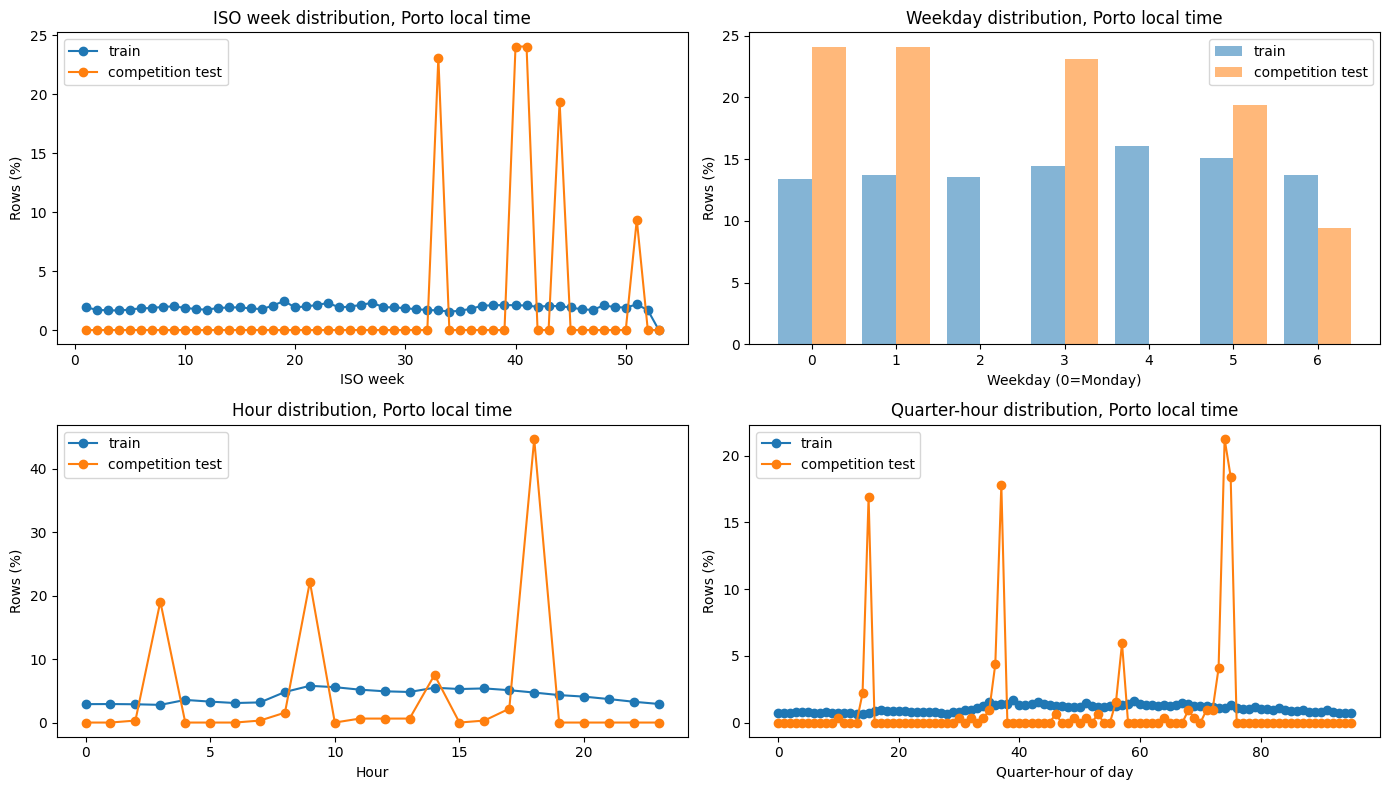
\includegraphics[width=\linewidth]{../outputs/dataset_analysis/plots/temporal_distributions.png}
  \caption[Temporal distributions of training trips and competition prefixes]{Temporal distributions of the training trips and the 320 competition prefixes in Porto local time.  The competition inputs are concentrated in later ISO weeks and a small set of observation times, motivating calendar features and caution when transferring results from a shuffled validation split.}
\end{figure}

\subsection{Cleaning and validation split}

We parse each polyline and remove incomplete, invalid, or shorter-than-two-point trajectories.  We then apply two conservative training-only checks: the first and final coordinates must fall inside a broad region around Porto, and GPS streams longer than four hours are removed only when they remain within 20~km of their start.  These steps remove 36,518 invalid or incomplete rows, 1,109 spatial outliers, and 142 duration artifacts, leaving \num{1672901} trajectories (97.792\% of the raw data).

Before feature construction, we create a shuffled 80/20 split with seed 42.  The resulting validation design contains \num{1338320} training rows and \num{334581} holdout rows.  Encoders, frequency statistics, and coordinate scaling are fitted on the training partition and then applied unchanged to the holdout.  For the final submissions, the same transformations are refitted on all retained trajectories.

\subsection{Competition-aligned synthetic prefixes}

The models must learn from complete training trajectories but predict from partial test trajectories of very different lengths.  We therefore generate one synthetic prefix per retained row in each partition:

\begin{enumerate}
  \item sample a desired length $L$ from the 320 supplied test-prefix lengths;
  \item select a training trajectory containing more than $L$ points;
  \item use its first $L$ points as input and its final point as target; and
  \item assert that the destination point is not present in the prefix.
\end{enumerate}

The supplied test trajectories were available during the competition, whereas their destinations and public/private membership were hidden.  Matching only their observable length distribution is therefore a competition-aligned use of the test inputs, not target leakage.  It produces synthetic prefixes with a median length of 26 points and a 95th percentile of 152 points, close to 26.5 and 152.15 in the test set.  A uniform cut-point strategy would instead produce much shorter examples, especially in the upper tail (\cref{fig:prefix-lengths}).  Seeds 42 and 43 generate the validation-training and validation-holdout prefixes; seed 142 generates a distinct full-data sample for final fitting.

\begin{figure}[H]
  \centering
  \begin{minipage}{0.88\linewidth}
    \centering
    \includegraphics[width=\linewidth]{prefix_length_quantiles.png}
    \caption[Observed prefix-length quantiles]{Observed prefix-length quantiles.  The selected synthetic strategy follows the supplied test-prefix distribution much more closely than uniform cutting.  The vertical axis is logarithmic.}
    \label{fig:prefix-lengths}
  \end{minipage}
\end{figure}

\subsection{Fixed-width representation}

Each variable-length prefix becomes a fixed-width feature row.  We retain the first five and last five observed points in chronological order, giving 20 standardized coordinate features.  Short prefixes are padded with their edge coordinate.  We add 12 numerical features: caller missingness and log frequency, prefix length, local week, weekday, 15-minute quarter of day, and sine/cosine encodings of the three time cycles.

The default representation one-hot encodes \texttt{CALL\_TYPE}, \texttt{ORIGIN\_STAND}, and \texttt{TAXI\_ID}.  Its 541 columns decompose as
\begin{equation}
  20\ \text{GPS}+12\ \text{numeric}+3\ \text{call type}
  +64\ \text{stand}+442\ \text{taxi}=541.
\end{equation}
High-cardinality \texttt{ORIGIN\_CALL} is represented by missingness and log frequency rather than one-hot encoding.  CatBoost receives the same 32 numerical columns plus four native categorical variables---\texttt{CALL\_TYPE}, \texttt{ORIGIN\_CALL}, \texttt{ORIGIN\_STAND}, and \texttt{TAXI\_ID}---for 36 columns in total.  This gives all models the same spatial and temporal information while allowing CatBoost to use its native categorical treatment.
